\section{Besonderes elektronisches Anwaltspostfach}
Das Gesetz zur Förderung des elektronischen Rechtsverkehrs mit den Gerichten hatte die Modernisierung der Kommunikation mit der Justiz vorgeschrieben. ''[...] Damit soll zugleich der derzeit noch bestehende ''Flickenteppich'' beim elektronischen Rechtsverkehr innerhalb der einzelnen Bundesländer beseitigt und eine bundesweit flächendeckende elektronische Infrastruktur geschaffen werden. Das beA wird – ggf. nach einer kurzen Umstellungsphase – zu einer Effektivierung und Beschleunigung der Arbeitsabläufe innerhalb der Kanzlei führen. Mittelfristig wird die ausschließlich elektronische Kommunikation zu einer Verkürzung der Postlaufzeiten und einer Einsparung an Druck-, Papier- und Portokosten führen. [...]'' \textcite{bea:bea:praxis:qa}\footfullcite{bea:bea:praxis:qa} \\
Infolgedessen wurde durch die Neuregelung in der Zivilprozessordnung (kurz ZPO) und in anderen Verfahrensordnungen die elektronischen Zugangswege für die Anwaltschaft zur Justiz erweitert. Lediglich die Verfassungs- und die Strafgerichtsbarkeit bleiben ausgenommen. Dadurch wurde auch auf die geringe Akzeptanz und Verbreitung des bisher (un)genutzten EGVPs und auf die hohen Sicherheitsmängel von dessen Nachfolger, der De-Mail, reagiert. \\
Gemäß §31a der Bundesrechtsanwaltsordnung \textcite{bea:bea:brao31}\footfullcite{bea:bea:brao31} (kurz BRAO) ist die Bundesrechtsanwaltskammer (kurz BRAK) verpflichtet zum 01.01.2016 jedem zugelassenen Rechtsanwalt ein besonderes elektronisches Anwaltspostfach (kurz beA) einzurichten. Fortan soll jede elektronische Kommunikation von Anwälten untereinander und zu den Gerichten ausschließlich über dieses Postfach stattfinden. Damit löst das beA das bisher genutzte EGVP für Rechtsanwälte ab.

\subsection{Rechtliche Rahmenbedingungen}
Im Vorfeld wurde heftig über die rechtlichen Rahmenbedingungen diskutiert. Man wolle den elektronischen Rechtsverkehr \textit{fördern}. So solle festgelegt werden, dass es eine verbindliche Verpflichtung zur Benutzung des beA für Rechtswälte gibt. Allerdings sollten auch einige Gesetze entschärft werden. So plädierte man auf die Absenkung des extrem hohen Signaturniveaus und auf die Zulassung anderer sicherer Standards, wie zum Beispiel die organisationsbezogene elektronische Signatur. Weiterhin sollte den Ländern Zeit gewährt werden, um den elektronischen Rechtsverkehr (kurz ERV) flächendeckend und stufenweise einzuführen. Weitere Forderungen der BRAK - wie zum Beispiel der Verzicht auf Zustellungsnachweise von Anwälten, die Ersetzung von Papierbekanntmachungen und -veröffentlichungen durch Internetveröffentlichungen und die vorbehaltlose Zulassung unterschriftsloser gerichtlicher Dokumente, die auf Druckstraßen erstellt wurden, sind beim Gesetzgeber eingereicht worden. \\
Mit der Veröffentlichung der Artikel §31, §31a und §31b BRAO \textcite{bea:bea:brao31} wurden die generellen Anforderungen an das besondere elektronische Anwaltspostfach gesetzlich festgehalten. Darin ist zusammengefasst folgendes festgeschrieben:
\begin{itemize}
	\item Die BRAK ist dazu verpflichtet zum 01.01.2016 jedem zugelassenen Rechtsanwalt ein besonderes elektronisches Anwaltspostfach (kurz beA) einzurichten. Dazu wird es ein Verzeichnis geben, dass alle zugelassenen Rechtsanwälte enthält und vom Bundesministerium der Justiz geführt und gepflegt wird.
	\item Die BRAK stellt sicher, dass der Zugang zum beA durch ein sicheres Verfahren mit zwei voneinander unabhängigen Sicherungsmittel möglich ist.
	\item Mit dem Verlust der Zulassung erlischt auch die Zugangsberechtigung zum beA. Das Postfach des Anwalts wird außerdem gelöscht.
\end{itemize}

Um das besondere elektronische Anwaltspostfach sicher zu gestalten, sollten die typischen sicherheitstechnischen Aspekte beachtet werden. Vor allem die Authentizität einer Person im System und die Integrität einer jeden Nachricht müssen gewährleistet werden. Weitere wichtige Aspekt sind der Datenschutz der gesicherten Nachrichten und Dokumente im Postfach und das elektronische Empfangsbekenntnis, welches besonders bei der Einhaltung von Fristen bedeutsam ist. Genaue Details sind in der Zivilprozessordnung §130a \textcite{bea:bea:zpo130}\footfullcite{bea:bea:zpo130} festgehalten:

\begin{quote}
	\begin{center}
		\textbf{§ 130a} \\
		\textbf{Elektronisches Dokument}
	\end{center}
	(1) Soweit für vorbereitende Schriftsätze und deren Anlagen, für Anträge und Erklärungen der Parteien sowie für Auskünfte, Aussagen, Gutachten und Erklärungen Dritter die Schriftform vorgesehen ist, genügt dieser Form die Aufzeichnung als elektronisches Dokument, wenn dieses für die Bearbeitung durch das Gericht geeignet ist. Die verantwortende Person soll das Dokument mit einer qualifizierten elektronischen Signatur nach dem Signaturgesetz versehen. Ist ein übermitteltes elektronisches Dokument für das Gericht zur Bearbeitung nicht geeignet, ist dies dem Absender unter Angabe der geltenden technischen Rahmenbedingungen unverzüglich mitzuteilen. \\
	(2) Die Bundesregierung und die Landesregierungen bestimmen für ihren Bereich durch Rechtsverordnung den Zeitpunkt, von dem an elektronische Dokumente bei den Gerichten eingereicht werden können, sowie die für die Bearbeitung der Dokumente geeignete Form. Die Landesregierungen können die Ermächtigung durch Rechtsverordnung auf die Landesjustizverwaltungen übertragen. Die Zulassung der elektronischen Form kann auf einzelne Gerichte oder Verfahren beschränkt werden. \\
	(3) Ein elektronisches Dokument ist eingereicht, sobald die für den Empfang bestimmte Einrichtung des Gerichts es aufgezeichnet hat.
\end{quote}

Ein weiteres wichtiges Merkmal stellt hier die qualifizierte elektronische Signatur (qeS) dar. Sie wird benutzt, um eine elektronische Nachricht oder ein elektronisches Dokument zu signieren, somit elektronisch zu unterschreiben, sodass anhand der Signatur der Urheber der Nachricht eindeutig ermittelt werden kann. Dies erfüllt den Anspruch nach Authentizität. \\
Gemäß § 130a ZPO-neu \textcite{bea:bea:zpo130} können ab 2018 elektronische Dokumente entweder qualifiziert elektronisch signiert oder über einen anderen ''sicheren Übermittlungsweg'' bei Gericht eingereicht werden, wie zum beispielsweise über das besondere elektronische Anwaltspostfach. Voraussetzung für den Verzicht auf die qeS ist allerdings ein sicheres Anmeldeverfahren vor dem Versand.
\\
Laut ZPO §130d \textcite{bea:bea:zpo130} wird die bereits zuvor angesprochene Nutzungspflicht für Rechtsanwälte und Behörden gesetzlich festgeschrieben. Dadurch müssen diese Parteien das beA benutzen und können bei Verweigerung sogar rechtlich belangt werden. Diese Regelung tritt für Rechtsanwälte und Behörden mit dem 01.01.2016 (spätestens mit dem 01.01.2022) in Kraft.

\begin{quote}
	\begin{center}
		\textbf{§ 130d} \\
		\textbf{Nutzungspflicht für Rechtsanwälte und Behörden}
	\end{center}
	Vorbereitende Schriftsätze und deren Anlagen sowie schriftlich einzureichende Anträge und Erklärungen, die durch einen Rechtsanwalt, durch eine Behörde oder durch eine juristische Person des öffentlichen Rechts einschließlich der von ihr zur Erfüllung ihrer öffentlichen Aufgaben gebildeten Zusammenschlüsse eingereicht werden, sind als elektronisches Dokument zu übermitteln. Ist dies aus technischen Gründen vorübergehend nicht möglich, bleibt die Übermittlung nach den allgemeinen Vorschriften zulässig. Die vorübergehende Unmöglichkeit ist bei der Ersatzeinreichung oder unverzüglich danach glaubhaft zu machen; auf Anforderung ist ein elektronisches Dokument nachzureichen.
\end{quote}

Allerdings wird keine Nutzungspflicht für Gerichte in §130d ZPO \textcite{bea:bea:zpo130} beschrieben. Für die Justiz gibt es derzeit keine entsprechende gesetzliche Verpflichtung. Den Ländern soll zunächst die Möglichkeit gegeben werden, für die betroffenen Gerichtsbarkeiten/Gerichtszweige die notwendigen Infrastrukturen und technischen Ausstattungen zu schaffen.

\subsection{Zeitplan}
Der folgende Zeitplan ist aus dem BRAKMagazin 2/2015, April 2015\textcite{bea:bea:brak2-2015} \footfullcite{bea:bea:brak2-2015} entnommen.
\begin{itemize}
\item \textbf{2016:} Am 1.1.2016 wird das beA-System mit etwa 165.000 Anwaltspostfächern in Betrieb genommen. So sieht es das Gesetz zur Förderung des elektronischen Rechtsverkehrs mit den Gerichten (ERV-Gesetz) vor. [...]
\item \textbf{2018:} Ab 2018 sollen alle Gerichte der Zivil-, Arbeits-, Finanz-, Verwaltungs- und Sozialgerichtsbarkeit für die elektronische Kommunikation über das beA erreichbar sein. Allerdings besteht für die Länder die Möglichkeit, diesen Zeitpunkt um ein oder zwei Jahre nach hinten zu verschieben.
\item Ab \textbf{Anfang 2018} können Dokumente über das beA auch \textbf{ohne} qualifizierte elektronische Signatur versendet werden. Außerdem kann ab 2018 ein elektronisches Empfangsbekenntnis über das beA versendet werden.
\item \textbf{2022:} Spätestens ab 1.1.2022 wird die Anwaltschaft verpflichtet sein, elektronisch mit der Justiz zu kommunizieren. Die Länder haben unter bestimmten Voraussetzungen die Möglichkeit, die obligatorische Nutzung des beA um ein oder zwei Jahre für jede Gerichtsbarkeit separat vorzuverlegen.
\item \textbf{Ausnahme:} Strafgerichtsbarkeit: Für die Strafgerichtsbarkeit läuft derzeit das Gesetzgebungsverfahren zur Einführung der elektronischen Akte im Strafverfahren. Der dort vorgeschlagene Zeitplan orientiert sich an den Regelungen des ERV-Gesetzes.
\end{itemize}

\subsection{Umsetzung des beA}
Das besondere elektronische Anwaltspostfach wurde im Zuge des Gesetzes zur Förderung des elektronischen Rechtsverkehrs beschlossen. Im neusten BRAKMagazin vom Juni 2015 \textcite{bea:bea:brak3-2015} \footfullcite{bea:bea:brak3-2015} ist nun ein großer Bericht mit neuen Einzelheiten und den ersten Bildern zur Benutzeroberfläche erschienen. \\
Das besondere elektronische Anwaltspostfach gleicht an sich den herkömmlichen E-Mail-Systemen. Allerdings bringt es besondere Sicherheit durch spezielle Authentifizierungsmechanismen, sichere Ende-zu-Ende-Verschlüsselung und elektronische Signaturen mit. Weiterhin sind die Funktionalitäten an die Anwaltstätigkeit angepasst. Um auf sein persönliches Postfach zuzugreifen kann entweder der Web-Client oder - falls vorhanden, die verknüpfte Kanzleisoftware benutzt werden. Das Postfach gleicht im Aussehen den Clients bekannter E-Mail-Anbieter, wie zum Beispiel Googlemail, Gmx oder Web.de.

\begin{center}
	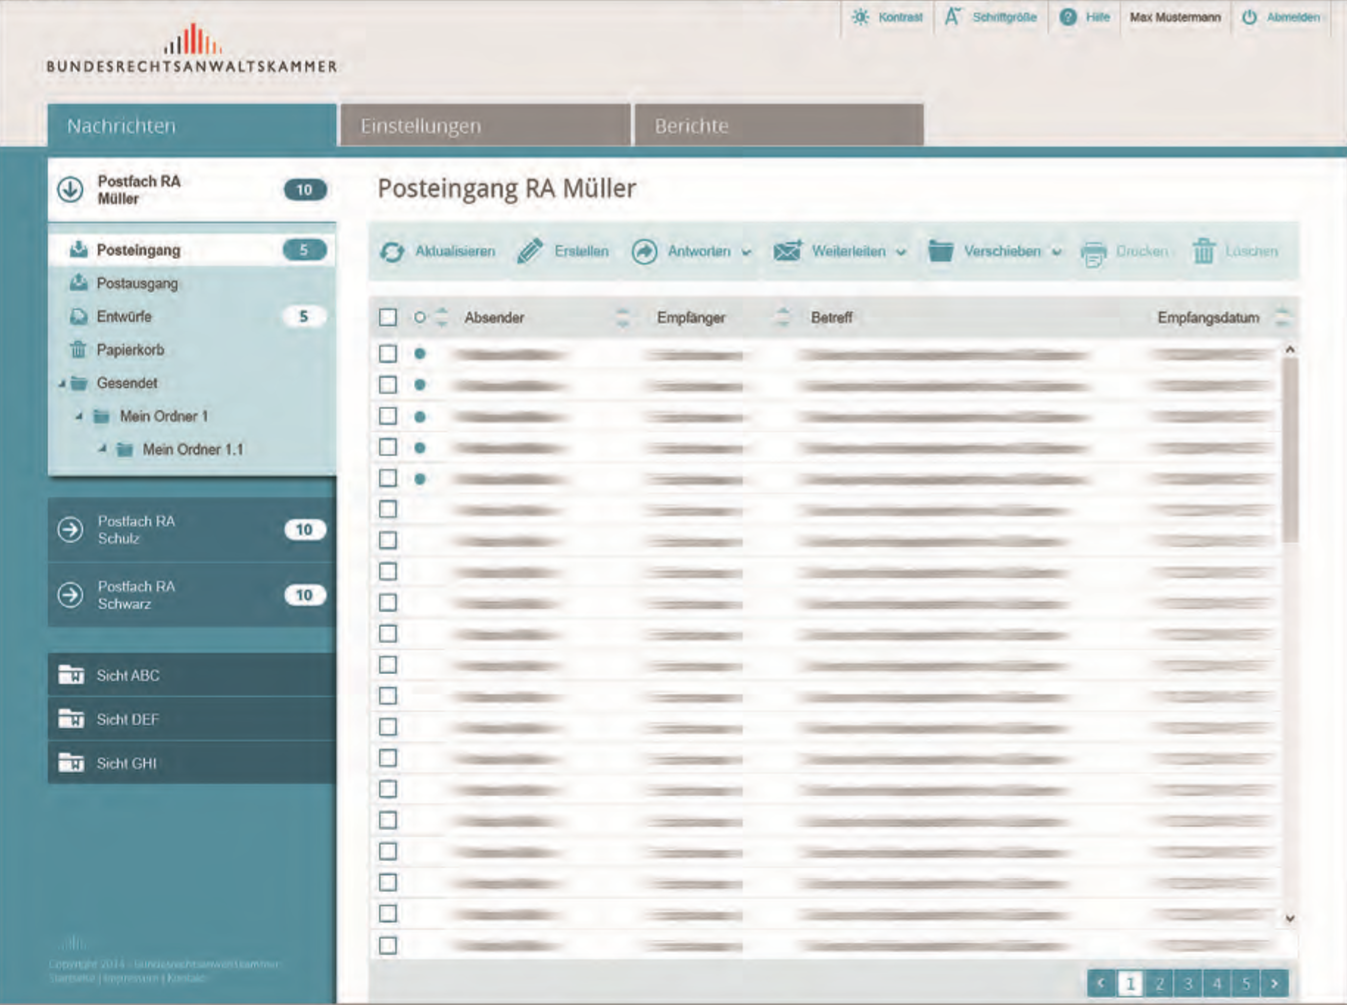
\includegraphics[width=\textwidth]{beA-ui1.png}
	\label{bea:gui:overview}
\end{center}

In Abbildung \ref{bea:gui:overview} ist die vorläufige Oberfläche des beA zu sehen. Man findet die typischen Ordner Posteingang und -ausgang, Entwürfe, Papierkorb und Gesendet vor, auf die der angemeldete Nutzer Zugriff hat. Beim beA kann der jeweilige Rechtsanwalt nur sein eigenes Postfach einsehen. Allerdings kann man Mitarbeitern bestimmte Rechte zuweisen, damit diese beispielsweise den Posteingang sehen und lesen können. Dadurch ist es auch möglich Urlaubsvertretungen festzulegen. Insgesamt wird es mehr als 30 Rechte geben, die man als Postfachinhaber an andere vergeben kann. Darunter fallen Lese-Rechte für bestimmte Ordner, das Recht Nachrichten zu versenden oder sogar das Recht, Rechte an andere vergeben zu dürfen. Durch dieses Rechte-System soll das geforderte jedoch nicht umgesetzte Kanzlei-Postfach simuliert werden. \\
''[...] Einen Wermutstropfen gibt es allerdings: Ein separates Kanzlei- oder Sozietätspostfach wird es nicht geben. Der Gesetzgeber wollte eine eindeutige Adressierbarkeit des einzelnen Rechtsanwaltes gewährleisten und hat daher in der BRAO festgelegt, dass nur Rechtsanwälte ein Anwaltspostfach erhalten. Um hier aber für anwaltliche Organisationseinheiten dennoch ein komfortables Arbeiten zu ermöglichen, gibt es so genannte Sichten (siehe Abbildung \ref{bea:gui:sichten}), die frei definierbar sind. Beispielsweise ist postfachübergreifend die Ansicht aller ungelesenen Nachrichten einstellbar, so dass eine Mitarbeiterin auf einen Blick alle neuen Nachrichten aus allen Postfächern, für die sie zugriffsberechtigt ist, sehen kann. So entsteht faktisch ein ''virtuelles Kanzleieingangspostfach''. Niemand muss sich durch alle Postfächer einzeln durchklicken. [...]''\textcite{bea:bea:brak3-2015} \\
Allerdings können nur Rechte für Personen vergeben werden, die auch im Verzeichnis des beAs zu finden sind, demgemäß zugelassene Rechtsanwälte. In der Realität wird die Post eines Anwalts in Kanzleien meist nicht verwaltet, es gibt Sekretäre oder Sekretärinnen, die sich darum kümmern. Meist handelt es hierbei nicht um zugelassene Rechtsanwälte, weshalb sie auch keinen Zugriff auf das besondere elektronische Anwaltspost haben und damit auch keine Rechte zugewiesen bekommen können. Dies wird sich in der Praxis durch die hohen Sicherheitsvorkehrungen gewiss als hinderlich erweisen.

\subsection{Wie werden Nachrichten versendet?}
Das Versenden einer Nachricht gleicht dem einer E-Mail. Aufgrund der Ende-zu-Ende-Verschlüsselung ist der Nachrichtenbetreff nicht einsehbar, da er auch verschlüsselt wird. Lediglich die Identität des Absenders und das Datum kann man im Klartext lesen. Wurde die Nachricht seitens des Empfängers einmal geöffnet und damit entschlüsselt, ist der Betreff lesbar. Wird sie hiernach geschlossen, wird der Nachrichten-Inhalt inklusive aller Anhänge abermals verschlüsselt, der Betreff bleibt fortan in der Nachrichtenübersicht lesbar. Die Ursache hierfür ist der zweistufige Sicherheitscontainer des Sicherheitsprotokolls OSCI, welches für das Verschlüsseln der Nachrichten verantwortlich ist. Hier werden Inhalts- und Nutzungsdaten streng voneinander getrennt und können dadurch kryptographisch unterschiedlich behandelt werden. Dies ist vor allem für die Datenvermittlung notwendig.\textcite{bea:osci} \footfullcite{bea:osci} Weitere Details über das Sicherheitsprotokoll OSCI sind im Kapitel \ref{sec:bea:sicherheit:osci} zu finden. \\
Nachrichten liegen niemals unverschlüsselt im beA-System vor. Eingegangene Nachrichten können wie bei herkömmlichen E-Mail-Clients nach Belieben sortiert werden, um so schnellsten Zugriff und Übersicht zu erreichen.
Eine weitere wichtige Neuerung ist das elektronische Empfangsbekenntnis. Ab Anfang 2018 wird es dieses als maschinenlesbaren Datensatz geben, der automatisch ausgestellt, zurückgeschickt und anschließend eingelesen werden kann. Bis dahin kann ein Empfangsbekenntnis auf dem normalen Weg - sprich per Post oder Fax, oder qualifiziert elektronisch signiert als Anhang einer beA-Nachricht verschickt werden. 

\begin{figure}[ht]
	\subfigure[Sichten im Postfach]{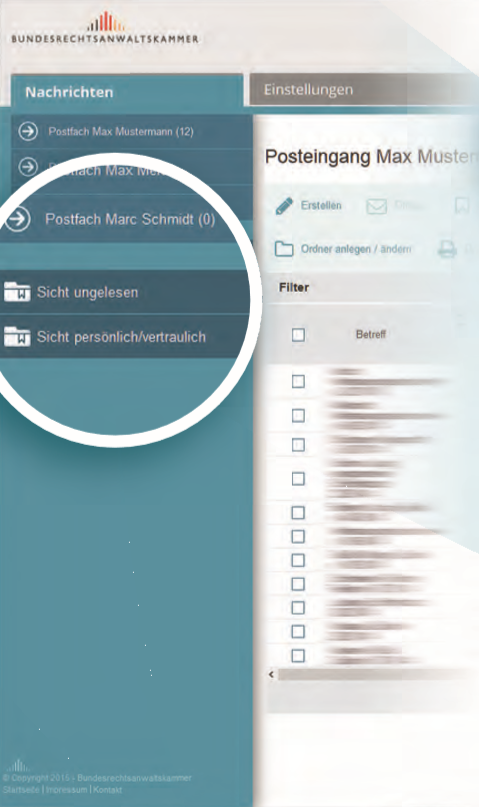
\includegraphics[width=0.49\textwidth]{beA-ui2.png}}
	\subfigure[Postfächer]{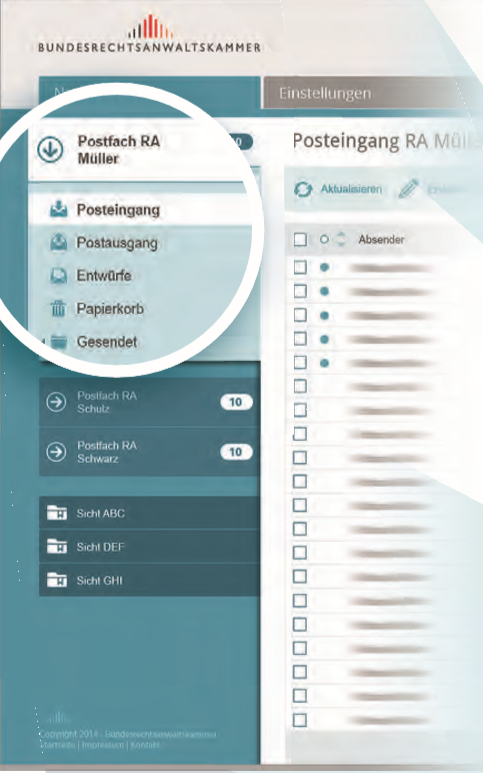
\includegraphics[width=0.49\textwidth]{beA-ui3.png}}
	\caption{Die Navigation innerhalb des Postfachs}
	\label{bea:gui:sichten}
\end{figure}


\subsection{Nachrichten versenden und weiterbearbeiten}
Der Versand der beA-Nachrichten gestaltet sich recht einfach. Es gibt ein Adressverzeichnis, in dem alle Gerichte, Rechtsanwälte, Kammern und sonstigen Empfänger, die über das beA erreicht werden können, aufgelistet sind. Dabei ist zu beachten, dass noch nicht alle Gerichte das beA ab dem 01.01.2016 unterstützen werden. \\
Die Absenderzeile wird vom System automatisch ausgefüllt. Für die maschinelle Verarbeitung und Struktur ist es möglich das eigene und das gerichtliche Aktenzeichen und das der Gegenseite anzugeben. Diese Daten werden beispielsweise als Nutzungsdaten behandelt und dadurch vom OSCI-Standard anders verschlüsselt, als der Nachrichteninhalt. Folglich sind sie - wie bereits im vorigen Kapitel erwähnt, nach dem ersten Entschlüsseln sichtbar. Typischerweise können auch Anhänge zur Nachricht hinzugefügt werden. ''[...] In der Regel wird es sich dabei um Schriftsätze und deren Anlagen handeln. Bezüglich der Nachrichtengröße und der Anzahl der Anhänge orientiert sich das beA an den Vorgaben der Justiz, die voraussichtlich der Hauptadressat von beA-Nachrichten sein wird. Da eine Nachricht gleichzeitig an mehrere Empfänger adressiert werden kann, z.B. an ein Gericht und einen Anwalt, kann für die Kommunikation zwischen Rechtsanwälten nichts anderes gelten. Nach den Vorgaben des Justizstandards dürfen Nachrichten derzeit nicht größer als 30MB sein und nicht mehr als 100 Anhänge umfassen. Die Erweiterung auf 150 MB und 500 Anhänge ist bereits beschlossen. Die verwendbaren Dateiformate richten sich nach den Rechtsverordnungen der Länder, das beA macht hier keine Vorgaben. Einschränkungen wird es nur bei Dateiendungen geben, die eindeutig auf eine Schadsoftware hinweisen. [...]'' \textcite{bea:bea:brak3-2015} \\
Am 01.01.2018 tritt der neue § 130a ZPO \textcite{bea:bea:zpo130} in Kraft. Dann können Nachrichten über das \textit{besondere elektronische Anwaltspostfach} auch ohne qualifizierte elektronische Signatur (kurz qeS) verschickt werden. Hier gilt zu beachten, dass für die Übertragung der Nachricht zu einem Gericht ein sicherer Übermittlungsweg gewählt wird. Das beA stellt einen solchen Weg dar. Allerdings muss die Nachricht vom Postfachinhaber selbst abgeschickt worden sein. Hat ein Mitarbeiter das Recht erlangt, Nachrichten in einem anderen Postfach zu versenden, muss diese Nachricht trotz allem qualifiziert elektronisch signiert werden, um zu jeder Zeit den Absender eindeutig identifizieren zu können. \\
Bis zu diesem Zeitpunkt werden Nachrichten ohne qeS gar nicht erst verschickt werden können. Dafür soll bei der Umsetzung des beA Sorge getragen werden. \\
\\
Eingegangene Nachrichten können - wie bei herkömmlichen E-Mail-Clients, beantwortet oder zu einem anderen beA-Postfach weitergeleitet werden. Zudem kann man Nachrichten ausdrucken oder exportieren. Das beA ist, aufgrund der benötigten Kapazität und damit verbundenen Kosten, kein Nachrichtenarchiv. ''[...] Nachrichten sollten daher nicht im beA belassen werden, sondern in regelmäßigen Abständen in das eigene Dateiablagesystem exportiert oder ausgedruckt und gelöscht werden. Die BRAK wird voraussichtlich innerhalb des ersten Jahres nach Inbetriebnahme des beA-Systems Fristen festlegen, nach deren Ablauf der Postfachinhaber darüber informiert wird, dass Nachrichten automatisch in den Papierkorb verschoben und später dann gelöscht werden. [...]'' \textcite{bea:bea:brak3-2015}

\subsection{Sicherheitstechnische Mittel}
Sicherheit - heißt Vertraulichkeit, Integrität, Authentizität, Verfügbarkeit und Verbindlichkeit, hat beim ERV und damit beim beA oberste Priorität. Findet ein Datenaustausch zwischen zwei Parteien statt, so soll gewährleistet werden, dass beide Parteien ihren Gegenüber eindeutig identifizieren können, kein Dritter den Datenaustausch manipulieren oder im Klartext lesen und dass der Austausch der Daten eindeutig den beiden Parteien zugeordnet werden kann. Dazu werden verschiedene sicherheitstechnische Mittel verwendet, die im Folgenden erläutert werden.

\subsubsection{Ende-zu-Ende-Verschlüsselung}
Vertraulichkeit und Integrität werden durch die sogenannte Ende-zu-Ende-Verschlüsselung einer beA-Nachricht gewährleistet. Bei dieser Verschlüsselung werden die Daten beim Sender verschlüsselt und erst beim Empfänger entschlüsselt. Dadurch können keine anderen Parteien während der Übertragung den Nachrichteninhalt im Klartext lesen. Um sich gegen sogenannte Man-In-The-Middle-Attacken zu schützen, generieren beide am Datenaustausch teilnehmenden Parteien einen String-Identifier, der auf ihren PublicKeys beruht. Dieser Identifier wird untereinander ausgetauscht. Stimmt der ausgetauschte mit dem eigenen überein, so kann davon ausgegangen werden, dass niemand die Kommunikation belauscht. Jedoch bleiben bei einer solchen Ende-zu-Ende-Verschlüsselung dennoch Risiken: die beiden Endpunkte. Wurde der eigene Computer infiziert, so können Angreifer den PrivateKey stehlen, der zur Entschlüsselung von übersandten Nachrichten benutzt wird. \\
Im Gegensatz zum Verschlüsselungssystem zur De-Mail können damit weder Administratoren noch die BRAK selbst Nachrichten auf dem Server mitlesen.

\subsubsection{Sicherheitskarte}
Die Sicherheitskarte stellt ein physisches Medium dar, auf dem Schlüssel zum Verschlüsseln oder elektronisch Signieren von Nachrichten aufbewahrt werden. Damit lassen sich zum Beispiel auch Login-Verfahren sichern, in dem die an den Server übermittelten Daten sowohl signiert als auch verschlüsselt werden können. Dies hat den Vorteil, dass Angreifer auch die Sicherheitskarte stehlen müssten. Man fügt so dem klassischen Authentifizierungsverfahren mittels Benutzerkennung und Passwort eine zweite Sicherheitskomponente hinzu. Um die Karte benutzen zu können, braucht man ein Kartenlesegerät und eine spezielle Kryptographie-Software auf dem Computer. Laut Gesetz zum beA muss dieses Kartenlesegerät ein Gerät mit eigener Eingabetastatur besitzen. Andernfalls könnten sogenannte KeyLogger, Programme, die die Tastaturanschläge aufzeichnen, die PIN für die Karte herausfinden und an Dritte übermitteln. Die Kryptographie-Software wird benutzt, um Nachrichten oder Dokumente zu verschlüsseln und entschlüsseln oder elektronisch zu signieren beziehungsweise eine elektronische Signatur zu überprüfen. Hierzu wird je ein paar von Schlüsseln benutzt, die verschieden sind, sich jedoch eindeutig einander zuordnen lassen. Dabei handelt es sich um einen privaten Schlüssel - den Signaturschlüssel, und einen öffentlichen Schlüssel - den Signaturprüfschlüssel. Der private Schlüssel bleibt geheim, während der öffentliche Schlüssel jedem zugänglich ist. Der Signaturprüfschlüssel ist eindeutig dem Besitzer zugeordnet. Eine Nachricht oder Dokument, welches vom privaten Schlüssel signiert wurde, kann nur mit dem öffentlichen Schlüssel überprüft werden. Dadurch kann der Absender einer signierten Nachricht immer eindeutig festgestellt werden. Wird der Inhalt während der Übertragung verändert, ändert sich damit auch die Prüfsumme der Nachricht und der Signaturprüfschlüssel schlägt fehl. Damit gewährleistet dieses Verfahren Authentizität und Integrität.

\subsubsection{S.A.F.E.}
Secure Access to Federated eJustice/E-Government (kurz S.A.F.E.) ist ein bundesweiter Dienst für die deutsche Verwaltung, der Anwendungen sichere elektronische Identitäten (eIDs) für Personen und Organisationen zur Verfügung stellt. Dadurch können diese Personen beziehungsweise Organisationen durch ihre eID eindeutig identifiziert werden. \textcite{bea:safe} \footfullcite{bea:safe} Diese eID gilt für alle Dienste, sogenannte Trust-Domains, die von S.A.F.E. anerkannt werden. Registriert man sich bei einem dieser Trust-Domains erhält man eine eID. Damit ist man auch bei allen anderen Trust-Domains mit dieser eID registriert. Das Netzwerk für die Kommunikation zu und zwischen Trust-Domains wird über etablierte Standards abgewickelt, wie zum Beispiel das OSCI-Protokoll. Das beA stellt eine solche Trust-Domain dar, jeder Rechtsanwalt hat seine eigene eID.

\subsubsection{OSCI}
\label{sec:bea:sicherheit:osci}
''OSCI-Transport (Online Services Computer Interface Transport) ist ein Protokollstandard zur vertraulichen und sicheren Übermittlung von Nachrichten in einer auf das deutsche Signaturgesetz abgestimmten Sicherheitsumgebung. OSCI steht dabei für mehrere Protokoll, deren gemeinsames Merkmal die besondere Eignung für das E-Government ist:
\begin{itemize}
	\item OSCI-Transport für die sichere, vertrauliche und rechtsverbindliche Übertragung digitaler Daten über das Internet sowie
	\item eine Reihe verschiedener Protokolle (OSCI-XÖV-Standards) für den Austausch fachlicher Inhaltsdaten auf XML-Basis zwischen Kunden und Behörden bzw. Behörden untereinander.'' \textcite{bea:osci}
\end{itemize}

OSCI-Transport-Nachrichten haben einen zweistufigen Sicherheitscontainer. Das bedeutet, dass Inhalts- und Nutzungsdaten voneinander getrennt und kryptografisch unterschiedlich zu behandelt werden können. Dabei werden beide Datensätze getrennt verschlüsselt. Danach werden sie in einen zweiten Sicherheitscontainer eingelegt, wobei dieser abermals verschlüsselt wird. Aufgrund dieses Prinzips spricht man in der Praxis auch oft vom ''Prinzip des Doppelten Umschlages''. Nachrichten werden immer Ende-zu-Ende-verschlüsselt. \\
Der Vorteil der Trennung von Inhalts- und Nutzungsdaten ist, dass der Intermediär nur die Nutzungsdaten sehen kann und damit auch zum Beispiel das beigefügte Aktenzeichen, wodurch dieser die Nachricht an die richtige Institution weiterreichen kann, ohne den tatsächlichen Inhalt lesen zu müssen. Die Inhaltsdaten können dadurch auch vom Nutzer eigenständig elektronisch signiert oder verschlüsselt werden, ohne, dass das System beeinträchtigt wird. \\
Jeder Sicherheitscontainer (für Nutzdaten und Inhaltsdaten) erlaubt die elektronische Signatur und die Verschlüsselung des jeweiligen Inhalts. Dadurch sind Vertraulichkeit, Integrität und Authentizität der Nachrichten gewährleistet. \textcite{bea:osci}

\subsubsection{Erstanmeldung}
Bevor ein Rechtsanwalt das besondere elektronische Postfach benutzen kann, muss sich dieser dort zuerst anmelden. Diese Erstanmeldung verknüpft das Postfach mit der Identität des Rechtsanwalts, weshalb dieser Vorgang besonders sicherheitssensibel ist. Dazu benötigt er eine besondere beA-Karte, die die Postfachnummer als auch die eID enthält. Nach Inbesitznahme des Postfachs kann die beA-Karte auch zur täglichen Anmeldung genutzt werden.

\subsection{Das beA in der Praxis}
In den letzten Kapiteln haben wir das besondere elektronische Anwaltspostfach sowohl aus rechtlicher als auch aus technischer Sicht durchleuchtet und vorgestellt. In diesem Kapitel geht es um die Anwendung des Systems in der Praxis, wie gut sich das beA in den Alltag integriert und welche Vor- beziehungsweise Nachteile es mit sich bringt. \\
Durch den elektronischen Rechtsverkehr muss eine stete Erreichbarkeit der Dienste gewährleistet werden, damit auch bestimmte Fristen eingehalten werden können. Jedoch werden, wie bei jedem anderen Dienst auch, Wartungsarbeiten durchgeführt werden müssen. Zu dieser Zeit wird das System nicht verfügbar sein.
Ist die Übertragung eines elektronischen Dokuments aus technischen Gründen nicht möglich, bleibt die Übermittlung dennoch zulässig. Das Dokument muss folglich nachgereicht und es muss glaubhaft gemacht werden, dass eine Übermittlung nicht möglich gewesen ist (siehe § 130d S. 2 ZPO n. F.\textcite{bea:bea:zpo130}). \\
Eine ähnliche Situation bietet sich, falls ein elektronisches Dokument vom Gericht nicht verarbeitet werden kann. Nach der Übertragung wird dies dem Absender mitgeteilt und der Zeitpunkt dieser Einreichung gilt, solange der Absender glaubhaft machen kann, dass das nachgereichte Dokument mit dem zuvor übermittelten übereinstimmt (siehe § 130a Abs. 6 ZPO n.F). \\
\\
Zudem entstehen gegebenenfalls weitere Kosten, um das beA nutzen zu können. Laut der Bundesrechtsanwaltkammer bedarf es folgender Voraussetzungen:
\begin{itemize}
	\item eine leistungsfähige Internetverbindung (mind. 2mbit/s),
	\item ein Computer mit mind. 512 MB Arbeitsspeicher und AMD- oder Intel-Prozessor,
	\item das aktuelle Betriebssystem: Windows, MacOS oder Linux,
	\item (beA-)Signaturkarte und Kartenlesegerät \textbf{mit Tastatur} und
	\item Drucker und Scanner. \textcite{bea:bea:brak}
\end{itemize}
Da eine Datenrate von 2 Mbit/Sekunde leider noch nicht überall in Deutschland verfügbar ist, wurde der rechtliche Rahmen im ERV-Gesetz so gestaltet, dass bei nachgewiesener Unmöglichkeit einer elektronischen Übersendung zum Gericht auch ein konventioneller Versand möglich sein wird. Dennoch ist dieser Zustand unbefriedigend: Die BRAK wird sich deshalb auf allen politischen Kanälen für einen zügigen Ausbau des Breitbandnetzes einsetzen. Immerhin haben die Regierungsfraktionen in ihrer Koalitionsvereinbarung von 2013 versprochen, dass es bis 2018 in Deutschland eine flächendeckende Grundversorgung mit mindestens 50 Mbit/Sekunde geben soll. \\
\\
Um das beA effektiv in der Kanzlei einzusetzen, ist in der Regel ein Drucker, ein Scanner oder eine Kombination aus beiden erforderlich. Der Scanner sollte auf verschiedene Auflösungen einstellbar sein, so dass die Pixeldichte je nach Dokumententyp – Textdatei oder Bilddatei – individuell einstellbar ist. Eine geringere Auflösung bedeutet eine geringere Dateigröße und damit einen einfacheren Versand der Nachrichtenanhänge. \\
Sicher bedeuten diese Anschaffungen zunächst einmal einen gewissen finanziellen Aufwand für jede Kanzlei. Dem gegenüber stehen jedoch deutliche Ersparnisse bei den Papier- und Portokosten und vor allem auch langfristig Vereinfachungen in den alltäglichen Arbeitsabläufen. Dabei fügt sich das beA selbstverständlich umso besser in den Arbeitsalltag ein, je stärker die Kanzlei an sich digitalisiert ist. Auch wenn die Nutzung des beA eine elektronische Aktenführung nicht voraussetzt, bietet die Einführung doch eine gute Gelegenheit auch insgesamt über eine Digitalisierung der Kanzlei nachzudenken

\subsubsection{Anwälte}
Anwälte erhalten mit dem beA keine herkömmliche E-Mail-Adresse, sondern ihre Adressdaten liegen in einer Datenbank. Nachrichten werden direkt an den jeweiligen Rechtsanwalt oder das jeweilige Gericht geschickt.
Der Begriff des Anwaltspostfachs ist dabei irritierend. Das Postfach ist nicht öffentlich, sondern nur die Adresse innerhalb des Systems. Der Anwalt kann zudem keine Nachrichten an Personen schicken, die kein Anwaltspostfach besitzen. Eine Kommunikation mit dem Mandanten ist über das beA aus diesem Grund nicht möglich. Dies führt dazu, dass Rechtsanwälte zwangsläufig mindestens zwei Kommunikationsmittel parallel benutzen müssen. \\
Die Kosten für die Einrichtung der besonderen elektronischen Anwaltspostfächer werden im Ergebnis von der Anwaltschaft zu tragen sein. ''[...] Für die Entwicklung des beA und die Bereitstellung der Betriebsumgebung erhebt die BRAK für die Jahre 2014 und 2015 zusammen einen Beitrag von 63 Euro pro Rechtsanwalt, der 2015 von den Rechtsanwaltskammern eingezogen wird. Die Kammern finanzieren diesen Beitrag unterschiedlich – teilweise durch eine Erhöhung der Mitgliedsbeiträge, teilweise durch eine Umlage und teilweise durch einen Rückgriff auf das Vermögen der jeweiligen Kammer. Die Beschlüsse dazu werden in den jeweiligen Kammerversammlungen durch die Mitglieder gefasst. Über die Beitragshöhe in den Folgejahren entscheiden die Rechtsanwaltskammern jeweils im Frühjahr. [...]'' \textcite{bea:bea:brak}

\subsubsection{Kanzleien}
Die Einführung und Verpflichtung zur Nutzung haben auch Auswirkungen auf das Arbeiten in der Kanzlei. Das beA bietet eine Schnittstelle an, die die eventuell vorhandene Kanzleisoftware benutzen kann, um auf das Postfach zuzugreifen. Damit dies schlussendlich funktioniert, müssen die Kanzleien ihre internen Systeme und Strukturen auf die Benutzung des beA umstellen. Im Kapitel zur Umsetzung des beA haben wir bereits gesagt, dass es keine Kanzleipostfächer geben wird. Stattdessen können durch Rechtevergabe ''virtuelle Kanzleipostfächer'' erstellt werden. Das bedeutet, dass jede Kanzlei diese Postfächer zuerst erstellen muss, was zu erheblichem Mehraufwand führt.  
Das besondere elektronische Anwaltspostfach bringt andererseits auch Vorteile mit sich: Ein wesentlicher Vorteil ist der schnelle und sichere Datenaustausch mit Zustellungsnachweis. Durch die Eingangsbestätigung weiß der Anwalt, ob und wann die Nachricht bei Gericht angekommen ist. Außerdem können elektronische Strukturdaten, zum Beispiel Daten zu Aktenzeichen, mit dem Gericht ausgetauscht werden. Zudem können diese Strukturdaten automatisch von der Kanzleisoftware eingelesen und verarbeitet werden. Ein gutes Beispiel ist das automatische Auslesen von Fristen aus den Strukturdaten und Eintragen in den Kalender in der Kanzleisoftware. \\
Die elektronische Aktenführung bietet zudem eine enorme Flexibilität. Denn elektronische Akten sind praktisch von überall, wo ein Netzzugang vorhanden ist, abzurufen. Auch Akteneinsichten oder Verfahrensstandabfragen werden zukünftig elektronisch und praktisch sogar von zu Hause oder dem Arbeitsplatz aus, möglich werden. Insofern ist ein permanenter und ortsunabhängiger Zugriff möglich. Zukünftig wird der Anwalt oder Rechtssuchende durch den elektronischen Zugang auch nicht mehr an die Öffnungszeiten der Gerichte gebunden sein, sondern hat – ohne Wartezeiten –  zeitlich unbegrenzten Zugriff auf die einzusehenden Dokumente.
Effizientere Arbeitsweise und Kostenreduzierung: Eine Kosteneinsparung ergibt sich bereits daraus, dass Portokosten für das Versenden von Schriftsätzen etc. oder für die Anforderung von Akten entfallen – ebenso die Kosten für Versandumschläge und das Ausdrucken oder Kopieren der Akten und Schriftsätze. Außerdem führt eine elektronische Archivierung der Akten dazu, Akten- und Papierberge zu vermeiden. Somit müssen keine zusätzlichen Räumlichkeiten bereitgehalten werden, in denen die Akten aufbewahrt werden. Auch eine umständliche Suche im Aktenkeller entfällt künftig. \\
Eine elektronische Aktenführung ermöglicht zudem eine effektivere Mandatsbearbeitung, als es mit Papierakten möglich ist. Dadurch wird die Aktenbearbeitung effizienter und schneller, denn es steht ein elektronischer Workflow für Sortierung, Suchfunktion und systematische Erfassung von Akteninhalten zur Verfügung. Akteninhalte können dadurch schneller aufgefunden und bearbeitet werden.

\subsection{Schutzschriftenregister}
''Schutzschriften sind vorbeugende Verteidigungsschriftsätze gegen erwartete Anträge auf Arrest oder einstweilige Verfügung. Mit ihnen will der mögliche Antragsgegner erreichen, dass der Antrag zurückgewiesen wird, wenigstens aber verhindern, dass dem Antrag ohne mündliche Verhandlung entsprochen wird. Derzeit muss eine Schutzschrift bei jedem Gericht eingereicht werden, bei dem ein Antrag auf Arrest oder einstweilige Verfügung zu erwarten ist. Die Einreichung einer Schutzschrift bei einem Gericht hat nur Wirkung für dieses Gericht. Sind potentiell mehrere Gerichte zuständig, kann die Einreichung der Schutzschriften einen erheblichen Arbeits- und Sachaufwand bei Antragsgegnern und Rechtsanwälten, aber auch bei den Gerichten verursachen.'' \textcite{bea:bea:brak-schutzschriften} \footfullcite{bea:bea:brak-schutzschriften}

''Es wird ein zentrales, bundesweites elektronisches Schutzschriftenregister eingerichtet, bei dem die Einreichung einer Schutzschrift genügt, um alle Zivil- und Arbeitsgerichte zu erreichen. § 945a Absatz 2 Satz 1 der Zivilprozessordnung (ZPO) sowie § 62 Absatz 2 Satz 3 und § 85 Absatz 2 Satz 3 des Arbeitsgerichtsgesetzes (ArbGG), jeweils in der zum 1. Januar 2016 in Kraft tretenden Fassung des Gesetzes zur Förderung des elektronischen Rechtsverkehrs mit den Gerichten vom 10. Oktober 2013 (BGBl. I S. 3786), sehen deshalb vor, dass eine bei dem Register eingereichte Schutzschrift als bei allen Zivil- und Arbeitsgerichten der Länder eingereicht gilt. Die zentral hinterlegten Schutzschriften können von den Gerichten elektronisch abgerufen werden (§ 945a Absatz 3 Satz 1 ZPO). Die näheren Bestimmungen über die Einrichtung und Führung des Registers, über die Einreichung von Schutzschriften zum Register, über den Abruf von Schutzschriften aus dem Register sowie über die Einzelheiten der Datenübermittlung und -speicherung sowie der Datensicherheit und der Barrierefreiheit werden auf Grundlage des § 945b ZPO durch Verordnung geregelt.\textbf{Für Rechtsanwälte wird das Elektronische Schutzschriftenregister über das beA erreichbar sein.}'' \textcite{bea:bea:brak-schutzschriften}

\subsection{Besonderes elektronisches Notarpostfach}
Notare nutzen ab dem 01.01.2016 das besondere Notarpostfach. Dessen Bereitstellung liegt im Verantwortungsbereich der Bundesnotarkammer. Dabei gleicht das Notarpostfach dem beA. Bisher haben Notare ein Postfach im EGVP besessen. \textcite{bea:notarpostfach} \footfullcite{bea:notarpostfach}